% Projektbericht FOC-Framework – Teil Software
% Übersetzen: latexmk (siehe .latexmkrc) oder pdflatex -> biber -> pdflatex -> pdflatex
\documentclass[
  a4paper,
  11pt,
  ngerman,
  oneside,
  parskip=half,
  bibliography=totoc,
  listof=totoc,
  numbers=noenddot,
]{scrreprt}

% ---------------------------------------------------------------
% Präambel
% ---------------------------------------------------------------
\usepackage[T1]{fontenc}
\usepackage[utf8]{inputenc}       % ab LaTeX 2018 Standard, schadet nicht
\usepackage[ngerman]{babel}
\usepackage{lmodern}
\usepackage{microtype}
\usepackage{csquotes}

\usepackage[a4paper, left=30mm, right=25mm, top=25mm, bottom=30mm]{geometry}

% Mathematik, Einheiten
\usepackage{amsmath, amssymb}
\usepackage[locale=DE, per-mode=symbol]{siunitx}

% Tabellen, Abbildungen
\usepackage{graphicx}
\graphicspath{{img/}{../matlab/reports/img/}{../docs/img/}}
\usepackage{booktabs}
\usepackage{tabularx}
\usepackage{float}
\usepackage[font=small, labelfont=bf]{caption}
\usepackage{subcaption}

% Farben, Quelltext
\usepackage[dvipsnames]{xcolor}
\usepackage{listings}
\lstset{
  basicstyle=\ttfamily\small,
  breaklines=true,
  frame=single,
  numbers=left,
  numberstyle=\tiny\color{gray},
  keywordstyle=\color{NavyBlue}\bfseries,
  commentstyle=\color{ForestGreen},
  stringstyle=\color{BrickRed},
  showstringspaces=false,
  literate={ä}{{\"a}}1 {ö}{{\"o}}1 {ü}{{\"u}}1 {Ä}{{\"A}}1 {Ö}{{\"O}}1 {Ü}{{\"U}}1 {ß}{{\ss}}1,
}
\lstdefinestyle{matlab}{language=Matlab}
\lstdefinestyle{c}{language=C}

% Abkürzungen (printonlyused erst setzen, wenn im Text \ac{...} verwendet wird,
% sonst bricht die leere Liste die Übersetzung ab)
\usepackage{acronym}

% Literatur
\usepackage[backend=biber, style=numeric, sorting=none]{biblatex}
\addbibresource{literatur.bib}

% Verweise (hyperref zuletzt, cleveref danach)
\usepackage[hidelinks, pdfusetitle]{hyperref}
\usepackage[ngerman, noabbrev]{cleveref}

% ---------------------------------------------------------------
% Eigene Befehle
% ---------------------------------------------------------------
% Platzhalter / noch zu schreiben (im PDF rot sichtbar)
\newcommand{\offen}[1]{\textcolor{red}{[#1]}}
% Datei-, Skript- und Blocknamen
\newcommand{\datei}[1]{\texttt{#1}}
\newcommand{\skript}[1]{\texttt{#1}}
\newcommand{\block}[1]{\textsf{#1}}
% Verweis auf den Hardwareteil des Laborpartners
\newcommand{\hwteil}[1]{(siehe Hardwareteil, #1)}


% ---------------------------------------------------------------
% Angaben für das Deckblatt (anpassen)
% ---------------------------------------------------------------
\newcommand{\berichtTitel}{FOC-Framework für den modularen Frequenzumrichter CarpeDiem}
\newcommand{\berichtUntertitel}{Teil Software: modellbasierte Weiterentwicklung der Motorregler-Firmware}
\newcommand{\berichtAutor}{Jan Krüger}
\newcommand{\berichtPartner}{{Bruno Pesavento} (Teil Hardware)}
\newcommand{\berichtBetreuer}{Prof. Dr.-Ing. Arno Bergmann}
\newcommand{\berichtVeranstaltung}{Projektarbeit}
\newcommand{\berichtDatum}{\offen{Abgabedatum}}

\begin{document}

\pagenumbering{Roman}
\begin{titlepage}
  \centering
  {\large Hochschule Bochum\par}
  \vspace{1ex}
  {\large Projekt CarpeDiem\par}
  \vspace{4cm}
  {\LARGE\bfseries \berichtTitel\par}
  \vspace{1.5ex}
  {\Large \berichtUntertitel\par}
  \vspace{3cm}
  {\large Projektbericht\par}
  \vspace{1ex}
  \berichtVeranstaltung\par
  \vfill
  \begin{tabular}{ll}
    Verfasser:     & \berichtAutor \\
    Laborpartner:  & \berichtPartner \\
    Betreuung:     & \berichtBetreuer \\
    Abgabe:        & \berichtDatum \\
  \end{tabular}
\end{titlepage}

\chapter*{Kurzfassung}
\addcontentsline{toc}{chapter}{Kurzfassung}

\offen{Zum Schluss schreiben, ca.\ eine halbe Seite: Ausgangslage (Simulink-Modell der
Masterarbeit), Ziel (FOC-Framework, modellbasiert), wichtigste Ergebnisse
(Bibliothek mit Äquivalenznachweis, korrigierte Regler, MIL-Tests,
Codegenerierung, CAN/FOCP mit FOC Studio, Schutzfunktionen), Stand und Ausblick.}

Dieser Bericht behandelt ausschließlich die Software. Die Hardwarebefunde und
Messungen am Aufbau beschreibt der Hardwareteil des Projektberichts.

\tableofcontents
\chapter*{Abkürzungen}
\addcontentsline{toc}{chapter}{Abkürzungen}

\begin{acronym}[FOCP]
  \acro{ADC}{Analog-Digital-Umsetzer}
  \acro{CAN}{Controller Area Network}
  \acro{CSA}{Strommessverstärker (Current Sense Amplifier)}
  \acro{FOC}{feldorientierte Regelung (Field-Oriented Control)}
  \acro{FOCP}{FOC-Protokoll (Kommunikation FOC Studio -- Firmware über CAN)}
  \acro{GUI}{Graphical User Interface}
  \acro{ISR}{Interrupt-Service-Routine}
  \acro{IPC}{Inter-Processor Communication}
  \acro{JTAG}{Joint Test Action Group (Debug-Schnittstelle)}
  \acro{MA}{Masterarbeit}
  \acro{MIL}{Model-in-the-Loop}
  \acro{PI}{Proportional-Integral(-Regler)}
  \acro{PU}{Per Unit (normierte Größe)}
  \acro{PWM}{Pulsweitenmodulation}
\end{acronym}


\cleardoublepage
\pagenumbering{arabic}
\chapter{Einleitung}
\label{ch:einleitung}

\section{Motivation und Aufgabenstellung}
Grundlage der Projektarbeit ist ein Frequenzumrichter, welcher 2023 von zwei Masterstudent der Hochschule Bochum modellbasiert entwickelt wurde. Initiale Aufgabe war es einen Anwendungsfall für den Frequenzumrichter zu realisieren.
Nach erster Bestandsaufnahme und Sichtung der Masterarbeiten stand jedoch schnell fest, dass zunächst die Firmware und Hardware überarbeitet werden muss.
Perspektivisch soll der Frequenzumrichter Firmen als Plattform für ihre eigene Entwicklung bereitgestellt werden können.

Aus dieser neu formulierten Aufgabenstellung heraus wurde das Ziel neu definiert: Ausbau des bestehenden Projekts hin zu einem FOC-Framework bestehend aus:

\begin{itemize}
	\item Wiederverwendbare C und MatLab Simulink Bibliothek für Anwendungsfälle
	\item Parametrisierung von Motoren über austauschbare Motorprofile 
	\item Ausbau der modellbasierten Tests
	\item Erstellung einer \ac{GUI}-Anwendung für die Inbetriebnahme und Bedienung des Frequenzumrichters über \ac{CAN}
\end{itemize}
\offen{Überarbeiten}

\section{Abgrenzung und Aufteilung im Team}
Dieser Projektbericht umfasst die Softwareseite der Projektarbeit.
Konkret werden die Themen Modelle, Skripte, Konfugirationen, generierter Code sowie Firmware-Anbindung über das entwickelte \ac{FOCP} und die Software "FOC Studio".

Nicht behandelt wird die Hardware, also Platine, Messungen, Hardware-Review und Befunde und Inbetriebnahme-Messungen.
% - Dieser Teil: Modelle, Skripte, Konfiguration, generierter Code,
%   Firmware-Anbindung FOCP, PC-Software FOC Studio
% - Hardwareteil (Laborpartner): Platine, Messungen, Hardware-Review
%   (HW-Befunde), Inbetriebnahme-Messungen. Hier nur Verweise darauf.
\offen{Querverweise, Überarbeiten}

\section{Aufbau des Berichts}
\offen{Kurzer Überblick über die Kapitel}
Im Kapitel \ref{ch:ausgangslage} wird zunächst die Ausgangslage, also der vorgefundene Stand der Masterarbeiten von 2023 beschrieben und die Befunde aus der Modellanalyse erläutert.

\ref{ch:vorgehen} stellt die modellbasierte Entwicklung und die verwendeten Werkzeuge vor. Es wird außerdem auf die Konfiguration über Profile und die Versionsverwaltung eingegangen.

Die Überführung des Simulink Modells aus den Masterarbeiten in eine wiederverwendbare Komponentenbibliothek wird in \ref{ch:bibliothek} dargestellt.

Der vorgefundene Regler wies einige Fehler auf. Die Korrektur dieser Befunde behandelt \ref{ch:regler}.

Wie diese Korrekturen durch Model-in-the-Loop-Tests verifiziert wurden ist in \ref{ch:verifikation} beschrieben.

Wie der generierte Quellcode auf die Hardware übertragen wurde und welche Besonderheiten dabei beachtet werden müssen ist in \ref{ch:codegen} festgehalten.

Die Kommunikation mit dem Frequenzumrichter wurde zunächst nur über \ac{CAN} realisiert. Das darunter liegende Protokoll \ac{FOCP} und die aufgetretenen Probleme werden in \ref{ch:kommunikation} diskutiert.

Um den Antrieb gegen Störsignale und kritische Betriebszustände abzusichern, wurden zusätzliche Schutz- und Robustheitsfunktionen ergänzt, darunter eine Begrenzung des Bremsstroms, eine Sollwert-Totzone und eine Überspannungsabschaltung. Diese werden in \ref{ch:schutz} zusammengefasst.

Für die Bedienung des Antriebs am PC wurde die Software FOC Studio entwickelt. \ref{ch:focstudio} dokumentiert ihre Anforderungen, Architektur und Funktionen sowie Test und Auslieferung.

Abschließend zieht \ref{ch:fazit} ein Fazit und benennt die offenen Punkte, die in weiterführenden Arbeiten adressiert werden sollten.

\chapter{Ausgangslage}
\label{ch:ausgangslage}

Grundlage dieser Arbeit sind zwei Masterarbeiten, die 2023 an der Hochschule Bochum
parallel entstanden sind: die Hardware des Frequenzumrichters \cite{darici2023} und die
modellbasiert entwickelte Firmware \cite{akguel2023}. Dieses Kapitel beschreibt den
vorgefundenen Stand aus Sicht der Software. Es stellt zunächst das Zielsystem vor, soweit
es für das Verständnis der Firmware nötig ist, dann das Simulink-Modell der Masterarbeit
und schließlich die Befunde, die sich bei der Analyse dieses Modells ergeben haben. Diese
Befunde bestimmen die Reihenfolge der späteren Arbeitsschritte.

% ---------------------------------------------------------------
\section{Zielsystem im Überblick}
\label{sec:zielsystem}

Der Frequenzumrichter besteht aus drei Baugruppen (\cref{fig:zielsystem}):

\begingroup\sloppy
\begin{description}
  \item[Steuerplatine] Eigenentwicklung aus \cite{darici2023} mit einem
    \textbf{TMS320F28386D} \cite{ti_f2838x_dm}. Der Baustein
    enthält zwei C28x-Kerne (CPU1, CPU2) mit je \SI{200}{\mega\hertz} und einen
    Arm-Cortex-M4-Kern, den \ac{CM}, für Ethernet, der über \ac{IPC} Daten mit den C28x-Kernen
    austauscht. Die Firmware läuft ausschließlich auf CPU1.
    Den Systemtakt erzeugt ein externer \SI{25}{\mega\hertz}-Oszillator. Über USB-C stellt
    ein FT2232HL eine \acs{JTAG}-Debugschnittstelle und eine serielle
    Schnittstelle bereit, über einen galvanisch getrennten Transceiver ist \ac{CAN}
    herausgeführt.
  \item[Leistungsstufe] Das zugekaufte \ac{EVM} \textbf{DRV8300DIPW-EVM}
    \cite{ti_slvubv6} mit dreiphasiger MOSFET-Brücke, Gatetreiber DRV8300, drei
    Low-Side-Shunts mit \ac{CSA}, Temperatursensor und dem Anschluss für die
    Hall-Sensoren. Es ist über zwei Stiftleisten im Raster des LaunchPads F280049C mit
    der Steuerplatine verbunden.
  \item[Motor] Der Motor ist ein permanentmagneterregter Synchronmotor vom Typ \textbf{ebm-papst ECI~63.60} \cite{ebmpapst_eci6360}. Er ist
     für \SI{24}{\volt} ausgelegt und besitzt vier Polpaare. Drei digitale Hall-Sensoren ermöglichen eine Lageerfassung der Ausgangswelle.
\end{description}
\endgroup

\begin{figure}[htbp]
  \centering
  \begin{tikzpicture}[
      node distance=8mm and 14mm,
      box/.style={draw, rounded corners=2pt, align=center, minimum height=26mm,
                  text width=34mm, font=\small},
      sig/.style={-Latex, font=\scriptsize},
    ]
    \node[box] (mcu) {\textbf{Steuerplatine}\\TMS320F28386D\\CPU1: Regelung\\
      \SI{25}{\mega\hertz} ext.\ Oszillator};
    \node[box, right=22mm of mcu] (evm) {\textbf{DRV8300DIPW-EVM}\\Gatetreiber\\
      B6-Brücke\\3 Shunts + CSA};
    \node[box, right=14mm of evm, text width=22mm] (mot) {\textbf{ECI 63.60}\\PMSM\\
      4 Polpaare\\Hall A/B/C};
    \node[box, below=10mm of mcu, minimum height=9mm] (pc) {PC / Bedienung};
    \node[box, below=10mm of evm, minimum height=9mm] (psu) {Labornetzteil
      \SI{24}{\volt}};

    \draw[sig] ([yshift=8mm]mcu.east) -- node[above]{6$\times$ PWM} ([yshift=8mm]evm.west);
    \draw[sig] ([yshift=-1mm]evm.west) -- node[above]{$i_a, i_b, i_c$, PVDD}
      ([yshift=-1mm]mcu.east);
    \draw[sig] ([yshift=-9mm]evm.west) -- node[above]{Hall, Temp.} ([yshift=-9mm]mcu.east);
    \draw[sig] ([yshift=4mm]evm.east) -- node[above]{$u_{abc}$} ([yshift=4mm]mot.west);
    \draw[sig] ([yshift=-6mm]mot.west) -- node[below]{Hall} ([yshift=-6mm]evm.east);
    \draw[Latex-Latex, font=\scriptsize] (pc) -- node[right]{CAN, USB (JTAG/UART)} (mcu);
    \draw[sig] (psu) -- node[right]{PVDD} (evm);
  \end{tikzpicture}
  \caption{Aufbau des Zielsystems mit den für die Firmware relevanten Signalen}
  \label{fig:zielsystem}
\end{figure}

Die für die Firmware wichtigen Peripherien sind in \cref{tab:peripherie} zusammengefasst.
Die drei Brückenzweige werden von ePWM6 bis ePWM8 angesteuert, mit \SI{20}{\kilo\hertz}
im Up-Down-Zählbetrieb (mittensymmetrische \ac{PWM}). Die Totzeit erzeugt der Gatetreiber,
nicht der Mikrocontroller. Eine Besonderheit des DRV8300\textbf{DI} ist, dass er die
Low-Side-Eingänge INLx invertiert. Der Mikrocontroller gibt deshalb auf ePWMxA und ePWMxB
dasselbe Signal aus. ePWM6 startet zugleich die Wandlung der Phasenströme, und zwar dann,
wenn die Low-Side-Schalter leiten und die Shunts den Strom sehen. Der Interrupt am Ende
dieser Wandlung ruft die Stromregelung auf. Damit ist die Stromregelung fest an die
\ac{PWM}-Periode von \SI{50}{\micro\second} gekoppelt.

\begin{table}[htbp]
  \centering
  \caption{Von der Firmware der \ac{MA} genutzte Peripherie (CPU1)}
  \label{tab:peripherie}
  \small
  \begin{tabularx}{\linewidth}{@{}>{\raggedright}p{36mm}>{\raggedright}p{34mm}
      >{\raggedright\arraybackslash}X@{}}
    \toprule
    Funktion & Peripherie & Bemerkung \\
    \midrule
    Brückenansteuerung & ePWM6/7/8 (GPIO10--15) & \SI{20}{\kilo\hertz}, Periode 5000 Takte \\
    Phasenströme $i_a$, $i_b$ & ADCINB0, ADCINB2 & Trigger ePWM6-SOCA, Interrupt ADCB1 $\to$ Stromregelung \\
    Phasenstrom $i_c$ & ADCINB3 & verdrahtet, aber nicht genutzt \\
    Zwischenkreisspannung, GVDD & ADCINA5, ADCINC3 & Unterspannungserkennung \\
    MOSFET-Temperatur & ADCINC2 & TMP23x, Übertemperatur \\
    Drehzahlsollwert & ADCINA0 & Potentiometer \\
    Hall A/B/C & eCAP1--3 (GPIO24--26) & Interrupt bei jedem Flankenwechsel \\
    SafeState-Taster & GPIO30 & Not-Aus in Software \\
    Kommunikation & eCAN-A, IPC zum CM & CAN-Kommandos, Ethernet-Logging über den CM \\
    \bottomrule
  \end{tabularx}
\end{table}

Einige Eigenschaften der Hardware wirken sich unmittelbar auf die Software aus. Dazu
zählen die Speisung der ADC-Referenz aus der \SI{3,3}{\volt}-Schaltreglerschiene und die
nur eingeschränkt realisierbare Überstromabschaltung in Hardware. Die Analyse dieser
Eigenschaften ist Gegenstand des Hardwareteils \hwteil{Hardware-Review}. Im vorliegenden
Bericht werden sie nur insoweit betrachtet, als sie Entwurf und Verhalten der Firmware
beeinflussen.

% ---------------------------------------------------------------
\section{Simulink-Modell der Masterarbeit}
\label{sec:impmodel}

Die Firmware der \ac{MA} \cite{akguel2023} enthält keinen handgeschriebenen C-Code. Sie
wird vollständig mit Embedded Coder \cite{mw_ecoder} und dem C2000 Microcontroller Blockset
\cite{mw_c2000} aus dem Modell \datei{impmodel.slx} generiert (MATLAB R2023a). Die Parameter
(Motor, Leistungsstufe, Bezugsgrößen, Reglerverstärkungen, Abtastzeiten) liegen in der
Binärdatei \datei{params\_f2838.mat}. Beide Dateien sind im Repository unverändert unter
\datei{matlab/models/legacy/} abgelegt und dienen in dieser Arbeit als Referenz für alle
Vergleiche. \Cref{fig:impmodel} zeigt die oberste Modellebene.

\begin{figure}[htbp]
  \centering
  \begin{tikzpicture}[
      font=\footnotesize,
      sub/.style={draw, align=center, minimum height=12mm, text width=22mm,
                  font=\footnotesize\sffamily},
      irq/.style={draw, dashed, align=center, minimum height=9mm, text width=22mm,
                  font=\footnotesize\sffamily},
      aux/.style={draw, align=center, minimum height=7mm, text width=22mm,
                  font=\footnotesize\sffamily},
      sig/.style={-Latex},
      lab/.style={font=\scriptsize, align=center},
    ]
    % Hauptsignalfluss
    \node[sub] (in) {Input\\Controller};
    \node[sub, right=16mm of in] (spd) {Speed Control\\\scriptsize $T_s = \SI{0,5}{ms}$};
    \node[sub, right=16mm of spd] (trq) {Torque Controller\\\scriptsize $T_s = \SI{50}{\micro s}$};
    \node[sub, right=16mm of trq] (plant) {Inverter and\\Motor -- Plant\\Model};

    % Interruptgesteuerte Subsysteme
    \node[irq, above=14mm of trq] (cg) {Code\\Generation};
    \node[irq, above=14mm of spd] (hall) {Hall Sensor\\A / B / C};
    \node[irq, above=14mm of plant] (ipc) {IPC Write for\\eCAP INTs};

    % Initialisierung und Hilfsfunktionen
    \node[aux, below=12mm of in] (init) {System Initialize};
    \node[aux, below=12mm of spd] (off) {ADC Offset Function};
    \node[aux, below=12mm of plant] (hb) {Heartbeat LED};

    \draw[sig] (in) -- node[lab, above]{Sollwert,} node[lab, below]{Freemode} (spd);
    \draw[sig] (spd) -- node[lab, above]{$i_{dq,\mathrm{ref}}$,} node[lab, below]{Freemode} (trq);
    \draw[sig] ([yshift=3mm]trq.east) -- node[lab, above]{Tastgrade} ([yshift=3mm]plant.west);
    \draw[sig] ([yshift=-3mm]plant.west) -- node[lab, below]{$i_{ab}$, Lage} ([yshift=-3mm]trq.east);
    \draw[sig] (trq.south) -- ++(0,-5mm) -| node[lab, pos=0.25, below]{Drehzahl} (spd.south);
    \draw[sig] (cg) -- node[lab, right]{ADCB1} (trq);
    \draw[sig] (cg) -- node[lab, above]{eCAP1--3} (hall);
    \draw[sig, densely dotted] (hall) -- node[lab, right]{Data Stores} (spd);
  \end{tikzpicture}
  \caption{Vereinfachte oberste Ebene des Modells \datei{impmodel.slx} aus \cite{akguel2023}.
    Gestrichelt: durch Interrupts aufgerufene Subsysteme. Die Original-Modellansicht zeigt
    \cref{fig:impmodel_orig} im Anhang.}
  \label{fig:impmodel}
\end{figure}

\subsection{Struktur}

Das Modell gliedert sich in folgende Subsysteme:

\begingroup\sloppy
\begin{description}
  \item[\block{System Initialize}, \block{ADC Offset Function}] Initialisierung, unter
    anderem der Pull-up-Widerstände über direkte Registerzugriffe, und Kalibrierung des
    Stromsensor-Offsets aus acht Abtastwerten mit Plausibilitätsprüfung.
  \item[\block{Code Generation}] Die Hardware-Interrupts: ADCB1 ruft den
    \block{Torque Controller} auf, eCAP1 bis eCAP3 die Hall-Auswertung.
  \item[\block{Hall Sensor A/B/C}] Interrupt-Routinen je Hall-Signal. Sie lesen den
    Hall-Zustand, prüfen seine Gültigkeit und legen Zustand, Drehrichtung und Zeitstempel
    in globalen Data Stores ab.
  \item[\block{Input Controller}] Sollwert vom Potentiometer, Unterspannung,
    Übertemperatur, SafeState-Taster sowie die CAN-Kommandos \enquote{Freemode} und
    \enquote{speedMode}. Außerdem werden Zwischenkreis- und Gatetreiberspannung zyklisch
    über CAN gesendet.
  \item[\block{Speed Control}] Drehzahlregelung, Abtastzeit \SI{0,5}{\milli\second}. Sie
    enthält die Freemode-Logik (\block{Digital\_Freemode\_Check} und
    \block{Mechanical\_Freemode\_Check}), die Sollwertberechnung (\block{Speed calculator})
    und einen \ac{PI} als Drehzahlregler (\block{PI\_Controller\_Speed}). Ausgang ist der
    Stromsollwert $\boldsymbol{i}_{dq,\mathrm{ref}} = (0,\ i_{q,\mathrm{ref}})$.
  \item[\block{Torque Controller}] Die eigentliche \ac{FOC}. Sie wird alle
    \SI{50}{\micro\second} von der \ac{ISR} des \ac{ADC} aufgerufen und umfasst
    Stromerfassung und Skalierung, Lage und Drehzahl aus den Hall-Signalen, Clarke- und
    Park-Transformation, \acs{PI}-Stromregler für $d$ und $q$,
    Spannungsbegrenzung (\enquote{DQ-Limiter}), inverse Park-Transformation,
    Raumzeigermodulation und Umrechnung in Vergleichswerte der ePWM-Module.
  \item[\block{Inverter and Motor -- Plant Model}] Streckenmodell aus Wechselrichter
    (Mittelwertmodell) und Motor für die Simulation.
  \item[\block{IPC Write for eCAP INTs}, \block{Heartbeat LED}] Übertragung von Messwerten
    an den \ac{CM}-Kern, der sie über ein zweites Modell (\datei{TCP\_Server.slx}) per
    Ethernet an den PC sendet, sowie eine Blink-LED als Lebenszeichen.
\end{description}
\endgroup

Die Regelung ist eine klassische Kaskade aus äußerem Drehzahl- und innerem Stromregelkreis
ohne Feldschwächung ($i_{d,\mathrm{ref}} = 0$). Gerechnet wird in normierten Größen, angegeben in
\ac{PU}, überwiegend im Datentyp \texttt{single} oder \texttt{fixdt(1,32,17)}. Die
Reglerverstärkungen wurden nicht von Hand eingestellt, sondern mit der internen, nicht
dokumentierten Funktion \texttt{mcb.internal.SetControllerParameters} des Motor Control
Blockset aus den Motordaten berechnet.

Alle hardwarenahen Teile sind über Variantenblöcke doppelt ausgeführt: Die Variante
\texttt{sim} speist die Regelung aus dem Streckenmodell, die Variante \texttt{codegen}
aus den Treiberblöcken des C2000 Blocksets. Simulations- und Codegenerierungspfad teilen
sich also die Reglerlogik, nicht aber die Messkette. Diese Trennung wird bei der Diagnose
in \cref{ch:regler} eine Rolle spielen.

\subsection{Sicherheitslogik}

Die einzige Rückfallebene ist der \enquote{Freemode}: Alle Schalter der Brücke werden
geöffnet, der Motor läuft frei aus, und der Fehler des Drehzahlreglers wird auf null
gesetzt. Ausgelöst wird er durch Unterspannung, Übertemperatur (bis zum Neustart
gespeichert), ein CAN-Kommando oder den SafeState-Taster. Eine Überspannungs- oder
Überstromabschaltung gibt es nicht. Die Untergrenze des Drehzahlreglers ist fest auf
$-0{,}5$ gesetzt, was ein leichtes Bremsen erlaubt.

\subsection{Anforderungen und Tests}

Die \ac{MA} leitet aus einem Lastenheft neun Systemmodellanforderungen
(SW\_ANF\_01 bis SW\_ANF\_09) ab. Vier davon sind mit Simulink Test als \ac{MIL}-Tests an
Test-Harnesses im Modell abgesichert (\cref{tab:mil_ma}), alle vier bestanden. Die
feldorientierte Regelung selbst (SW\_ANF\_06) und die Hall-Auswertung (SW\_ANF\_09) sind
nur auf der Hardware gezeigt, nicht modellbasiert getestet. Die Testdatei
\datei{Testfile\_F2838.mldatx} ist Teil der \ac{MA}.

\begin{table}[htbp]
  \centering
  \caption{\ac{MIL}-Tests der \ac{MA} \cite{akguel2023}}
  \label{tab:mil_ma}
  \small
  \begin{tabularx}{\linewidth}{@{}llX@{}}
    \toprule
    Harness & Getesteter Block & Anforderung \\
    \midrule
    \texttt{Freemode\_Check\_TestHarness} & \block{Digital\_Freemode\_Check}
      & SW\_ANF\_01/07/08 (Freemode bei CAN, Unterspannung, Übertemperatur) \\
    \texttt{SafeState\_TestHarness} & \block{Mechanical\_Freemode\_Check}
      & SW\_ANF\_03 (SafeState-Taster) \\
    \texttt{MaxVel\_TestHarness} & \block{Speed calculator}
      & SW\_ANF\_04 (Höchstdrehzahl je speedMode) \\
    \texttt{SpeedController\_TestHarness} & \block{PI\_Controller\_Speed}
      & SW\_ANF\_05 (Drehzahlregler, Begrenzung) \\
    \bottomrule
  \end{tabularx}
\end{table}

\subsection{Was nicht übernommen werden konnte}

Zwei Teile des Ausgangsstands ließen sich nicht direkt weiterverwenden:

\begin{itemize}
  \item \textbf{Ethernet-Logging:} Weil die Ethernet-Pins auf der eigenen Platine anders
    belegt sind als auf der controlCARD des Herstellers, wurden in der \ac{MA} Dateien des
    C2000 Support Package geändert (Präprozessorschalter
    \texttt{CARPEDIEM\_PIN\_CORRECTION}). Diese Änderungen sind nicht Teil des Archivs.
    Außerdem verstößt eine Änderung an der Toolbox gegen die Reproduzierbarkeit des Builds.
    Die Ethernet-Strecke über den \ac{CM} wurde daher nicht weiterverfolgt; die
    Kommunikation läuft stattdessen über \ac{CAN} (\cref{ch:kommunikation}).
  \item \textbf{Zielprozessor:} Das Modell ist für den TMS320F28388D der controlCARD
    konfiguriert, auf der Platine sitzt der pinkompatible TMS320F28386D. Auch die
    Taktquelle in den Hardware-Einstellungen musste an den externen
    \SI{25}{\mega\hertz}-Oszillator angepasst werden (\cref{ch:codegen}).
\end{itemize}

% ---------------------------------------------------------------
\section{Befunde aus der Modellanalyse}
\label{sec:befunde}

Bevor das Modell umgebaut wurde, wurden Reglerblöcke, Parameterdatei und Messkette im
Detail untersucht. Die Ergebnisse sind in \cref{tab:befunde} als Befunde B1 bis B6
zusammengefasst. Sie werden im weiteren Bericht mit diesen Kürzeln referenziert.

\begin{table}[htbp]
  \centering
  \caption{Befunde aus der Analyse des Altmodells}
  \label{tab:befunde}
  \small
  \renewcommand{\arraystretch}{1.15}
  \begin{tabularx}{\linewidth}{@{}l>{\raggedright\arraybackslash}X
      >{\raggedright\arraybackslash}X >{\raggedright\arraybackslash}p{27mm}@{}}
    \toprule
    Nr. & Befund & Wirkung & Behandlung \\
    \midrule
    B1 & I-Anteil des Drehzahlreglers um Größenordnungen zu klein
       & praktisch P-Regler, bleibende Drehzahlabweichung
       & \cref{ch:regler} \\
    B2 & Stromregler: I-Anteil wie B1 zu klein, $K_p$ von Hand verändert,
         Ausgang auf $[0, 1]$ begrenzt
       & negative Stellspannung unmöglich
       & \cref{ch:regler} \\
    B3 & Motordaten um Faktoren neben dem Datenblatt
       & Auslegung und Streckenmodell passen nicht zum Motor
       & Profil \texttt{datasheet} (\cref{ch:vorgehen}) \\
    B4 & Strom-PU-Basis im Modell weicht von der Bezugsgröße ab
       & wirksame Reglerverstärkung anders als ausgelegt
       & \cref{ch:regler} \\
    B5 & Variable \texttt{dataType} fehlt in der Parameterdatei
       & Modell nicht ohne Zusatzschritt übersetzbar
       & \cref{ch:bibliothek} \\
    B6 & ADC-Referenz \SI{3,36}{\volt} statt \SI{3,3}{\volt}
       & \SI{1,8}{\percent} Verstärkungsfehler
       & Profil \texttt{datasheet} \\
    \bottomrule
  \end{tabularx}
\end{table}

\subsection*{B1 und B2: Integralanteil der Regler}

Am Block \block{PI\_Controller\_Speed} ist als Integralverstärkung
\texttt{Ki\_speed\_texas*Ts\_speed} eingetragen, gleichzeitig ist die Option
\texttt{UseKiTs} gesetzt. Die Variable \texttt{Ki\_speed\_texas} stammt aus
\texttt{SetControllerParameters} und ist bereits der Integralbeiwert je Abtastschritt in der
Form der TI-Bibliothek, also $T_s/T_n$ ohne $K_p$. Er wird im Block ein zweites Mal mit der
Abtastzeit multipliziert. Statt etwa $0{,}095$ je Schritt wirkt so ein Wert von etwa
$6{,}6 \cdot 10^{-6}$. Der Drehzahlregler arbeitet damit praktisch als reiner P-Regler mit
$K_p = 7{,}2$ und kann eine bleibende Regelabweichung nicht ausregeln.

Die beiden Stromregler im \block{Torque Controller} haben denselben Fehler im
Integralanteil. Dazu kommen zwei weitere Eingriffe: Der Proportionalbeiwert ist als
\texttt{Kp\_i - 0.0002} eingetragen, offenbar eine Handkorrektur, und der Reglerausgang ist
auf $[0, 1]$ begrenzt. Im Betrieb braucht die $d$-Achse aber eine negative Spannung, etwa
$u_d \approx -\omega L i_q$. Die Begrenzung verhindert das.

Ob \texttt{UseKiTs} bedeutet, dass der eingetragene Wert bereits $K_i T_s$ ist, oder dass der
Block intern mit $T_s$ multipliziert, ändert nur die Größe des Fehlers. In beiden Lesarten
ist der Integralanteil um mindestens drei Größenordnungen zu klein.

\subsection*{B3: Motordaten}

Die Motordaten in \datei{params\_f2838.mat} weichen deutlich vom Datenblatt ab
(\cref{tab:motordaten}). Die ältere Parameterdatei der \ac{MA} für das LaunchPad F280049C
enthält dagegen die Datenblattwerte. Aus Spannungskonstante und Leerlaufdrehzahl
(\SI{6000}{\per\minute} bei \SI{24}{\volt}) ergibt sich ein Polradfluss von etwa
\SI{5,9}{\milli\volt\second}. Widerstand und Induktivität im Datenblatt sind sehr
wahrscheinlich Werte zwischen zwei Klemmen, je Strang also die Hälfte. Die
Reglerverstärkungen der \ac{MA} sind aus den abweichenden Werten berechnet. Der
Proportionalbeiwert des Stromreglers ist dadurch etwa um den Faktor 500 kleiner als bei
Auslegung mit den Datenblattwerten. Motorparameter gemessen hat die \ac{MA} nicht: Der Autor
nennt das selbst als Schwachstelle \cite{akguel2023}.

\begin{table}[htbp]
  \centering
  \caption{Motordaten ECI~63.60: Parameterdatei der \ac{MA} und Ableitung aus dem
    Datenblatt \cite{ebmpapst_eci6360}}
  \label{tab:motordaten}
  \small
  \begin{tabular}{@{}lrr@{}}
    \toprule
    Größe & \datei{params\_f2838.mat} & aus Datenblatt, je Strang \\
    \midrule
    Strangwiderstand $R_s$ & \SI{9}{\milli\ohm} & \SI{22,5}{\milli\ohm} \\
    Induktivität $L_d = L_q$ & \SI{0,153}{\micro\henry} & \SI{38}{\micro\henry} \\
    Polradfluss $\Psi_\mathrm{PM}$ & \SI{0,69}{\milli\volt\second} & \SI{5,9}{\milli\volt\second} \\
    \bottomrule
  \end{tabular}
\end{table}

\subsection*{B4: Skalierung der Strommessung}

Die Bezugsgrößen des Modells (Struktur \texttt{PU\_System}) setzen
$I_\mathrm{base} = \SI{17,6}{\ampere}$ und $U_\mathrm{base} = \SI{20,78}{\volt}$ an, und mit
diesen Werten werden die Regler ausgelegt. Im Codegenerierungspfad wird der Strom aber
direkt als $(\text{ADC} - \text{Offset})/2048$ berechnet. Ein \ac{PU} ist dort also der
Strom, bei dem der Strommessverstärker \SI{1,65}{\volt} Hub liefert. \texttt{PU\_System}
kommt in diesem Pfad nicht vor. Der Parameter \texttt{ISenseVoltPerAmp}
(\SI{3}{\milli\volt\per\ampere}) berücksichtigt nur den Shunt, nicht die Verstärkung des
\ac{CSA} auf dem \ac{EVM}. Welcher Strom einem \ac{PU} tatsächlich entspricht und welches
Vorzeichen die Messung hat, war zu Beginn offen. Geklärt wurde das erst mit den Unterlagen
des \ac{EVM} \cite{ti_slvubv6, ti_slvc817} im Zuge der Reglerkorrektur
(\cref{ch:regler}).

\subsection*{B5 und B6: Parameterdatei und ADC-Referenz}

Das Modell verwendet eine Variable \texttt{dataType} zur Wahl zwischen Gleit- und
Festkommavarianten, die in \datei{params\_f2838.mat} fehlt. Ohne zusätzliches Anlegen dieser
Variable lässt sich das Modell nicht übersetzen. Die Referenzspannung der \ac{ADC} ist in den
Parametern mit \SI{3,3}{\volt} angesetzt. Auf der Platine hängt sie an der
\SI{3,3}{\volt}-Versorgung, die mit \SI{3,36}{\volt} gemessen wurde \cite{darici2023}. Alle
analogen Messwerte haben dadurch einen Verstärkungsfehler von \SI{1,8}{\percent}.

\subsection*{Weitere Auffälligkeiten}

Neben den Befunden B1 bis B6 fielen kleinere Unstimmigkeiten auf, die keinen eigenen
Arbeitsschritt erforderten, aber bei einer Weiterentwicklung zu beachten sind:

\begin{itemize}
  \item Der Hall-Lageoffset ist doppelt gepflegt: \num{0,411} in den Motorparametern,
    \num{0,38} fest im Block \block{Mechanical to Electrical Position}. Der Wert im Block
    wurde laut \ac{MA} experimentell ermittelt.
  \item Die Mailbox für das CAN-Kommando \enquote{speedMode} ist in der
    Schnittstellentabelle der \ac{MA} mit 10, im Modell mit 15 angegeben.
  \item Mehrere Anforderungstexte entsprechen nicht mehr dem Modell, zum Beispiel die
    Begrenzung des Drehzahlreglers in SW\_ANF\_05.
  \item Die \ac{IPC}-Blöcke senden ständig an den \ac{CM}-Kern, auch wenn dort kein Programm
    läuft. Das führte später auf der Hardware dazu, dass die Strom-\ac{ISR} hängen blieb
    (\cref{ch:kommunikation}).
\end{itemize}

\section{Folgerungen}
\label{sec:folgerungen}

Der Ausgangsstand ist eine lauffähige, in sich geschlossene Firmware mit einer
nachvollziehbaren Struktur und einem Grundstock an \ac{MIL}-Tests. Für eine
Weiterverwendung als Framework fehlt aber dreierlei: 
\begin{enumerate}
	\item Die Parameter sind nicht
	nachvollziehbar (Binärdatei, interne Auslegungsfunktion, Befunde B3 bis B6).
	\item Die Regler
	arbeiten nicht wie ausgelegt (B1, B2).
	\item Die Komponenten sind fest in ein einziges
	Anwendungsmodell eingebaut.
\end{enumerate}
 Daraus ergibt sich die Reihenfolge der folgenden Kapitel:
zuerst die Parameter aus Skripten bei bitgleichem Verhalten, dann die Aufteilung in eine
Bibliothek, erst danach die Korrekturen an den Reglern. Jede Korrektur wurde einzeln vorgenommen und in anschließend in der Simulation nachgewiesen.
Dadurch war es möglich die Korrektheit jeder Korrektur zu überprüfen bevor die nächste vorgenommen wurde.

\chapter{Vorgehen und Werkzeuge}
\label{ch:vorgehen}

\section{Modellbasierte Entwicklung}
% Embedded Coder, C2000 Microcontroller Blockset; Altmodell bleibt unveränderte Referenz
\offen{Text}

\section{Skriptgesteuerte Modelländerungen}
% Jede Änderung als Skript in matlab/tools (add_block, set_param, ...),
% Ausgabe vorher/nachher, ein Schritt = ein Commit, Tags P1a/P1b/P1b.1,
% Bericht je Schritt unter matlab/reports
\offen{Text, Beispiel-Listing eines Werkzeugskripts}

\section{Konfiguration und Profile}
% matlab/config, matlab/design: toolboxfrei (auch GNU Octave), foc_startup(Profil)
% Profile legacy_f2838 (bitgleich zur MA) und datasheet (Datenblatt, ausgelegte Regler)
% test_config als Selbsttest
\offen{Text, Tabelle der Profile}

\section{Versionsverwaltung und Nachvollziehbarkeit}
\offen{Text}

\chapter{Überführung in eine Komponentenbibliothek}
\label{ch:bibliothek}

\section{Parameter aus Skripten (P0)}
% params_f2838.mat -> foc_config, Behebung B5
\offen{Text}

\section{Bibliothek focLib und Anwendungsmodell app\_speed (P1a)}
% foc_build_library: Subsysteme als Bibliotheksblöcke, app_speed verknüpft sie
\offen{Text, Abbildung Struktur focLib / app\_speed}

\section{Äquivalenznachweis zum Altmodell}
% foc_check_equivalence / foc_equivalence_p1a: alle Abweichungen exakt 0;
% wird nach jeder späteren Änderung mit Profil legacy_f2838 wiederholt
\offen{Text, Ergebnistabelle}

\chapter{Korrektur der Regler}
\label{ch:regler}

Mit der Bibliothek aus \cref{ch:bibliothek} liegt ein Stand vor, der sich exakt wie das
Altmodell verhält. In diesem Kapitel werden die Befunde B1 und B2 an den Reglern behoben.
Dazu werden die Regler zunächst nachvollziehbar neu ausgelegt
(\cref{sec:auslegung}) und die Korrekturen einzeln in der Simulation bewertet
(\cref{sec:p1b}). Die erste Bewertung erfüllte alle vorab festgelegten Kennzahlen, zeigte in
den Zeitverläufen aber eine Dauerschwingung. Deren Ursache lag nicht im Regler, sondern in der
Messkette des Simulationsmodells (\cref{sec:grenzzyklus}). Nach deren Korrektur zeigt
\cref{sec:p1b1} das Ergebnis.

% ---------------------------------------------------------------
\section{Reglerauslegung}
\label{sec:auslegung}

Die \ac{MA} berechnet die Reglerverstärkungen mit einer internen Funktion des Motor Control
Blockset (\texttt{mcb.internal.\allowbreak SetControllerParameters}). Sie ist von Matlab nicht dokumentiert, ihre Ergebnisse
hängen von den fehlerhaften Motordaten ab (B3) und ihre Ausgabe ist in einer Form, die im
Modell zum Fehler B1 geführt hat. Sie wird deshalb durch das Skript
\skript{foc\_design\_controllers} ersetzt, das die Auslegung mit Standardverfahren offenlegt
und die Strukturfelder des Altmodells füllt.

\subsection{Stromregler}

Die Strecke des Stromregelkreises einer Achse besteht aus der Statorwicklung
(Widerstand $R_s$, Induktivität $L$) und einer Ersatztotzeit $\sigma$, die Rechentotzeit
($1\,T_s$) und die mittlere Verzögerung der \ac{PWM} ($0{,}5\,T_s$) zusammenfasst:
\begin{equation}
  G_i(s) = \frac{1/R_s}{1 + s\,L/R_s} \cdot \frac{1}{1 + s\,\sigma},
  \qquad \sigma = 1{,}5\,T_s .
\end{equation}
Ausgelegt wird ein \ac{PI}-Regler $K_p\,(1 + 1/(s T_n))$ nach dem Betragsoptimum. Die
Nachstellzeit kompensiert die elektrische Zeitkonstante, die Verstärkung ergibt sich aus der
verbleibenden Totzeit:
\begin{equation}
  T_n = \frac{L}{R_s}, \qquad K_p = \frac{L}{2\sigma}, \qquad K_i = \frac{K_p}{T_n}.
\end{equation}
Der geschlossene Kreis hat dann eine Durchtrittsfrequenz von etwa
$f_c \approx 1/(2\pi \cdot 2\sigma)$. Da der Motor Oberflächenmagnete hat
($L_d = L_q$), sind $d$- und $q$-Regler gleich.

\subsection{Drehzahlregler}

Unter der Annahme, dass der Stromregelkreis gegenüber dem Drehzahlkreis schnell ist, reduziert
sich die Strecke auf das mechanische System mit Drehmomentkonstante $K_t = 1{,}5\,p\,\Psi$ und
Trägheitsmoment $J$:
\begin{equation}
  G_n(s) = \frac{K_t}{J\,s}.
\end{equation}
Die Verstärkung wird aus einer gewählten Durchtrittsfrequenz $\omega_c$ bestimmt, die
Nachstellzeit als Vielfaches von deren Kehrwert:
\begin{equation}
  K_p = \frac{J\,\omega_c}{K_t}, \qquad T_n = \frac{4}{\omega_c}.
\end{equation}
Der Faktor 4 ergibt ohne Berücksichtigung der Totzeiten eine Phasenreserve von etwa
\SI{76}{\degree}. Das Überschwingen auf einen
Sollwertsprung liegt wegen der Nullstelle des \ac{PI}-Reglers dennoch bei etwa
\SI{15}{\percent}. Gewählt ist $f_c = \SI{5}{\hertz}$. Die Bandbreite ist bewusst klein gewählt: Die
Drehzahl wird aus den Hall-Signalen gewonnen, die bei vier Polpaaren nur 24 Flanken je
Umdrehung liefern. Bei \SI{200}{\per\minute} liegen zwischen zwei Flanken
\SI{12,5}{\milli\second}, was wie eine zusätzliche Messtotzeit wirkt.

\subsection{Umrechnung in normierte Größen}

Das Modell rechnet in \ac{PU}. Die Verstärkungen müssen daher mit den Bezugsgrößen
umgerechnet werden, und zwar mit denen, die im Modell tatsächlich wirken. Wie Befund B4 zeigt,
sind das nicht die Werte aus der Struktur \texttt{PU\_System} der \ac{MA}. Die Bezugsgrößen
werden deshalb in \skript{foc\_pu\_system} aus der Signalkette abgeleitet:

\begin{itemize}
  \item \textbf{Strom:} Im Modell gilt $i_\mathrm{PU} = (\text{ADC} - \text{Offset})/2048$.
    Ein \ac{PU} ist der Strom, der den \ac{ADC} um 2048 Stufen aus dem Offset auslenkt.
    Mit der Messkette des \ac{EVM} (\cref{sec:p1b1}) ergibt sich
    \begin{equation}
      I_\mathrm{base} = \frac{2048 \cdot U_\mathrm{ref}/4095}{R_\mathrm{shunt} \cdot G_\mathrm{CSA}}
      = \frac{2048 \cdot \SI{3,36}{\volt}/4095}{\SI{3}{\milli\ohm} \cdot 10}
      \approx \SI{56,0}{\ampere}.
    \end{equation}
  \item \textbf{Spannung:} Die Raumzeigermodulation setzt eine normierte Stellgröße von 1 in
    die Strangspannung $U_\mathrm{dc}/\sqrt{3}$ um, also
    $U_\mathrm{base} = \SI{24}{\volt}/\sqrt{3} \approx \SI{13,86}{\volt}$.
\end{itemize}

Die normierte Stromreglerverstärkung ist dann
$K_{p,\mathrm{PU}} = K_{p,\mathrm{SI}} \cdot I_\mathrm{base}/U_\mathrm{base}$, die des
Drehzahlreglers $K_{p,\mathrm{PU}} = K_{p,\mathrm{SI}} \cdot \omega_\mathrm{base}/I_\mathrm{base}$.
\Cref{tab:auslegung} fasst die Ergebnisse für das Profil \texttt{datasheet} zusammen.
\skript{test\_config} prüft die Auslegung, indem es die Verstärkungen in SI-Einheiten
zurückrechnet und den Betrag des offenen Drehzahlkreises bei $f_c$ auswertet.

\begin{table}[htbp]
  \centering
  \caption{Ausgelegte Reglerparameter (Profil \texttt{datasheet},
    $T_s = \SI{50}{\micro\second}$, $T_{s,n} = \SI{0,5}{\milli\second}$)}
  \label{tab:auslegung}
  \small
  \begin{tabular}{@{}lrrr@{}}
    \toprule
    Größe & SI & \ac{PU} & Bemerkung \\
    \midrule
    \multicolumn{4}{@{}l}{\textit{Stromregler ($d$ und $q$)}} \\
    $K_p$ & \SI{0,253}{\volt\per\ampere} & \num{1,031} & $L/(2\sigma)$ \\
    $T_n$ & \SI{1,69}{\milli\second} & & $L/R_s$ \\
    $K_i$ & & \SI{606}{\per\second} & $K_p/T_n$ \\
    $f_c$ & \SI{1,06}{\kilo\hertz} & & $1/(2\pi\cdot 2\sigma)$ \\
    \midrule
    \multicolumn{4}{@{}l}{\textit{Drehzahlregler}} \\
    $K_p$ & \num{0,0053}\,A/min$^{-1}$ & \num{0,380} & $J\omega_c/K_t$ \\
    $T_n$ & \SI{127}{\milli\second} & & $4/\omega_c$ \\
    $K_i$ & & \SI{2,99}{\per\second} & $K_p/T_n$ \\
    $f_c$ & \SI{5}{\hertz} & & gewählt \\
    \bottomrule
  \end{tabular}
\end{table}

% ---------------------------------------------------------------
\section{Korrektur der Reglerblöcke (P1b)}
\label{sec:p1b}

\subsection{Änderungen}

Die Korrekturen werden von \skript{foc\_apply\_fixes} in der Bibliothek ausgeführt, getrennt
für Strom- und Drehzahlregler (\cref{tab:fixes}). Beide stellen die PID-Blöcke auf eine
Integralverstärkung in \si{\per\second} um (\texttt{UseKiTs = off}). Damit gibt es nur noch
eine Interpretation des Parameters, und die Ursache von B1 entfällt unabhängig davon, wie
\texttt{UseKiTs} im Altmodell gemeint war.

\begin{table}[htbp]
  \centering
  \caption{Korrekturen an den PID-Blöcken durch \skript{foc\_apply\_fixes}}
  \label{tab:fixes}
  \small
  \begin{tabularx}{\linewidth}{@{}l>{\raggedright\arraybackslash}X
      >{\raggedright\arraybackslash}X@{}}
    \toprule
    Parameter & vorher (Altmodell) & nachher \\
    \midrule
    \multicolumn{3}{@{}l}{\textit{Stromregler $d$, $q$ (\texttt{current\_pi}, B2)}} \\
    $P$ & \texttt{Kp\_i - 0.0002} & \texttt{Kp\_i} \\
    $I$ & \texttt{Ki\_texas*Ts}, \texttt{UseKiTs = on} & \texttt{Ki\_i} in \si{\per\second},
      \texttt{UseKiTs = off} \\
    Ausgang & $[0,\ 1]$ & $[-1,\ 1]$ \\
    \midrule
    \multicolumn{3}{@{}l}{\textit{Drehzahlregler (\texttt{speed\_pi}, B1)}} \\
    $I$ & \texttt{Ki\_speed\_texas*Ts\_speed}, \texttt{UseKiTs = on}
      & \texttt{Ki\_speed} in \si{\per\second}, \texttt{UseKiTs = off} \\
    Ausgang & $[-0{,}5,\ 1]$ & unverändert (später parametriert, \cref{ch:schutz}) \\
    \bottomrule
  \end{tabularx}
\end{table}

\subsection{Versuchsplan}

Das Skript \skript{foc\_run\_p1b} simuliert drei Läufe mit dem Profil \texttt{datasheet}
über \SI{8}{\second}: Lauf A mit den unkorrigierten Reglern, Lauf B nach der Korrektur der
Stromregler und Lauf C nach zusätzlicher Korrektur des Drehzahlreglers. Der Drehzahlsollwert
springt bei $t = \SI{1}{\second}$ von 0 auf \SI{0,25}{PU}, das Streckenmodell ist mit
\SI{10}{\percent} des Nennmoments belastet. Ausgewertet werden vier Kennzahlen über die letzten
\SI{20}{\percent} des Laufs:

\begin{itemize}
  \item $\bar e_n$: mittlere Drehzahlabweichung, zeigt eine bleibende Regelabweichung,
  \item $e_{iq,\mathrm{rms}}$, $e_{id,\mathrm{rms}}$: Effektivwert der Stromregelabweichung
    je Achse,
  \item $u_{d,\min}$: kleinste $d$-Spannung über den gesamten Lauf, zeigt, ob die
    Begrenzung auf $[0, 1]$ aufgehoben ist.
\end{itemize}

Die Erwartungen wurden vor den Läufen festgelegt: In Lauf A ist $u_{d,\min} \geq 0$ und
$\bar e_n \neq 0$; in Lauf B ist $e_{iq,\mathrm{rms}}$ deutlich kleiner als in A; in Lauf C
gilt zusätzlich $\bar e_n \approx 0$.

\subsection{Ergebnis}

\Cref{tab:p1b} zeigt die Kennzahlen. Formal ist jede Erwartung erfüllt. Die Zeitverläufe
in \cref{fig:p1b_e0} zeigen jedoch, dass in den Läufen B und C die $d$-Spannung ab etwa
\SI{0,05}{\second} fast rechteckförmig zwischen $\pm 0{,}9$ springt, mit etwa
\SI{325}{\hertz} und bis zum Ende des Laufs. Der Wert $u_{d,\min} = -0{,}94$ ist also die
Amplitude einer Dauerschwingung und kein Beleg für eine sinnvoll genutzte negative
Spannung. Der niedrige Wert von $e_{iq,\mathrm{rms}}$ ergibt sich, weil der Sollwert im
eingeschwungenen Zustand klein ist. Erst $e_{id,\mathrm{rms}} = 0{,}23$ zeigt die Schwingung.

\begin{table}[htbp]
  \centering
  \caption{Kennzahlen P1b (\SI{8}{\second}, Auswertung \SIrange{6,4}{8}{\second})}
  \label{tab:p1b}
  \small
  \begin{tabular}{@{}lrrrr@{}}
    \toprule
    Lauf & $\bar e_n$ & $e_{iq,\mathrm{rms}}$ & $e_{id,\mathrm{rms}}$ & $u_{d,\min}$ \\
    \midrule
    A unkorrigiert & \num{0,188} & \num{0,233} & \num{0,0097} & \num{0} \\
    B + Stromregler & \num{-0,0037} & \num{0,074} & \textbf{\num{0,235}} & \num{-0,943} \\
    C + Drehzahlregler & \num{-0,000004} & \num{0,073} & \textbf{\num{0,235}} & \num{-0,943} \\
    \bottomrule
  \end{tabular}
\end{table}

\begin{figure}[htbp]
  \centering
  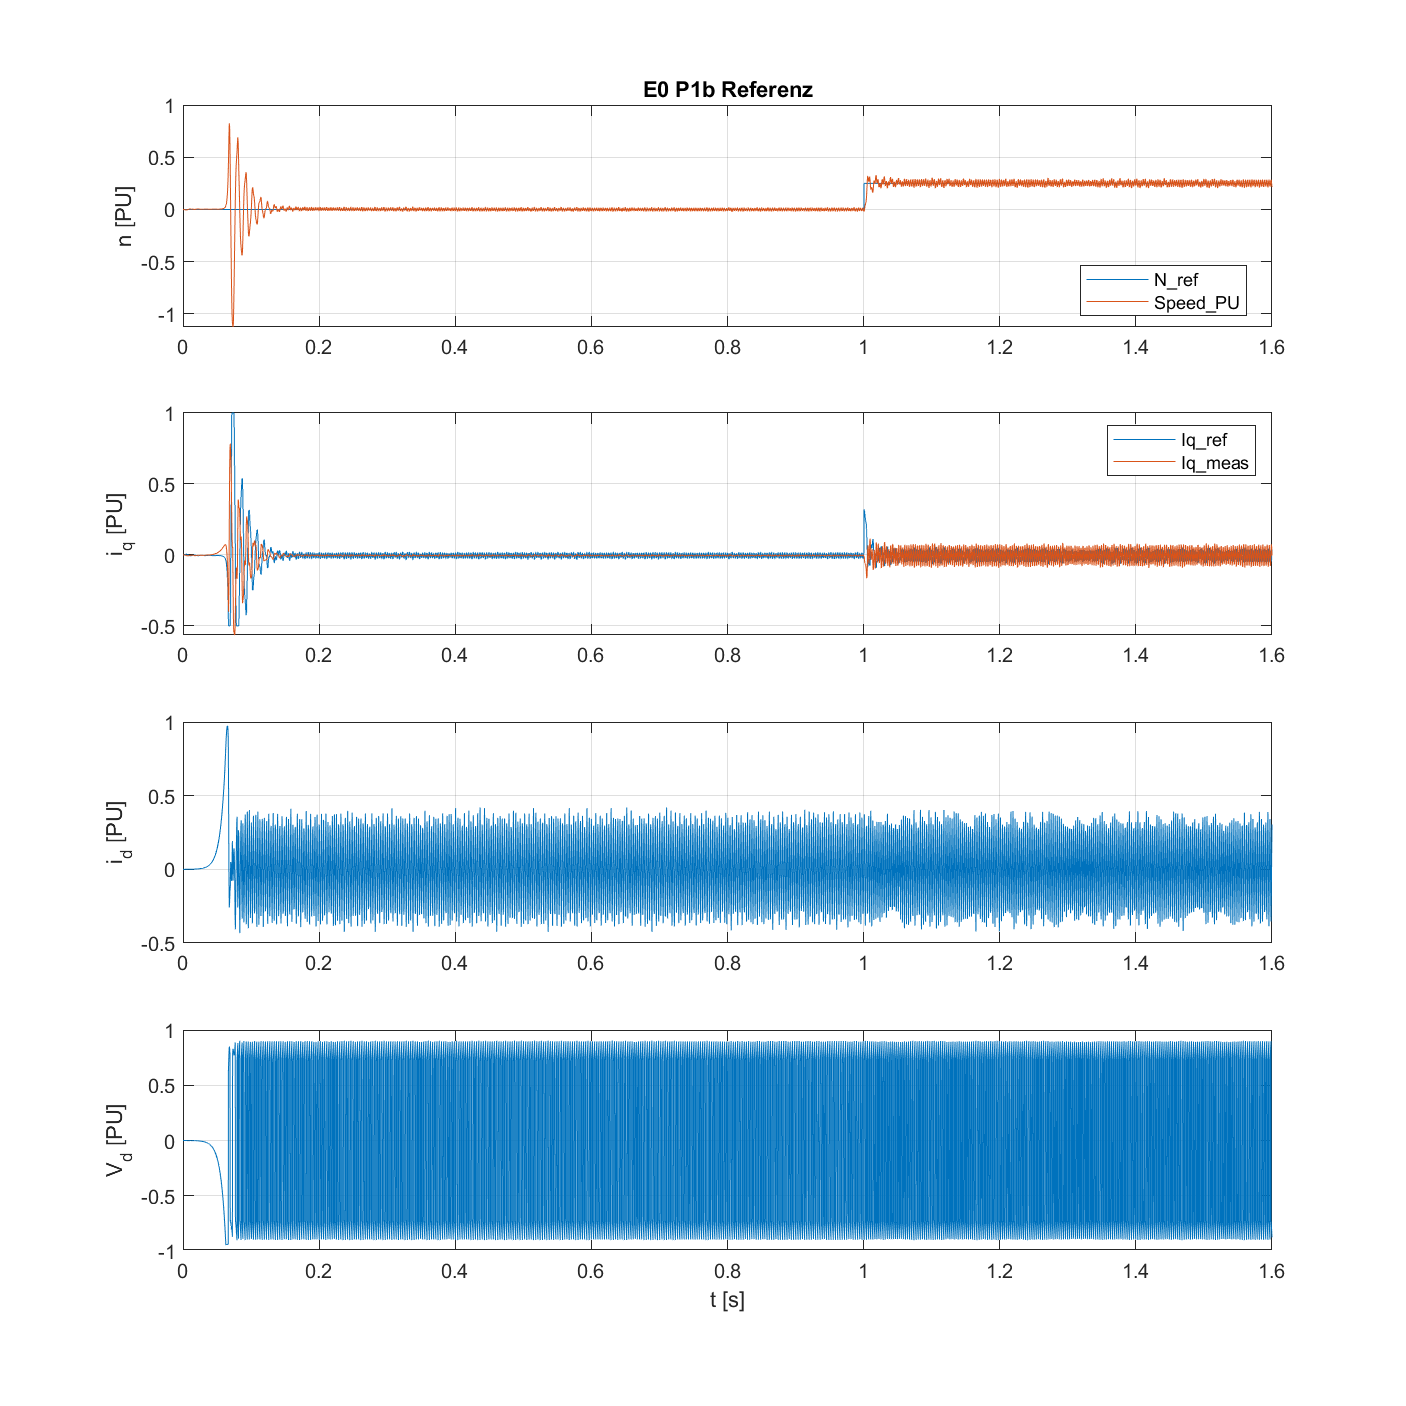
\includegraphics[width=0.9\linewidth]{P1b_diag_E0_P1b_Referenz}
  \caption{Stand P1b (korrigierte Regler, ursprüngliches Sensormodell): Drehzahl, $i_q$,
    $i_d$ und $u_d$ in \ac{PU}. Ab etwa \SI{0,05}{\second} schwingt der Stromregelkreis
    dauerhaft an der Stellgrößenbegrenzung.}
  \label{fig:p1b_e0}
\end{figure}

Der Stand wurde als \texttt{P1b} getaggt, um den Befund reproduzierbar zu halten, aber nicht
als hardwaretauglich freigegeben. Seitdem gehört zur Bewertung jedes Laufs die Sichtprüfung
der Zeitverläufe, insbesondere von $u_d$ und $i_d$.

% ---------------------------------------------------------------
\section{Diagnose des Grenzzyklus}
\label{sec:grenzzyklus}

Die Schwingung wurde nicht durch Nachstellen der Reglerparameter behandelt, sondern zunächst
rein lesend untersucht. Logging-Einstellungen wurden nur im Arbeitsspeicher gesetzt, die
Modelle nach jedem Lauf ohne Speichern geschlossen.

\subsection{Vorzeichen des Regelkreises}

Aus einer Simulation wurden die $d/q$-Größen aus Sicht des Reglers ($C$) und die
$d/q$-Größen der Strecke ($P$, Signale des Motorblocks) aufgezeichnet und per komplexer
Regression ins Verhältnis gesetzt:

\begin{itemize}
  \item Strompfad: $\underline{I}_C = k \cdot \underline{I}_P$ mit
    $|k| = \SI{560}{\ampere}/\mathrm{PU}$ und einer Drehung von \SI{-172,7}{\degree},
  \item Spannungspfad: $\underline{U}_C = k \cdot \underline{U}_P$ mit
    $|k| = \SI{14,7}{\volt}/\mathrm{PU}$ und einer Drehung von \SI{+7,2}{\degree}.
\end{itemize}

Ein reiner Fehler im Rotorwinkel würde beide Pfade um denselben Winkel mit
entgegengesetztem Vorzeichen drehen und sich im Kreis aufheben. Hier liegen die Drehungen
aber \SI{180}{\degree} auseinander. Wirksam ist damit $\underline{I}_C \approx -G \cdot
\underline{U}_C$: Der Stromregelkreis ist \textbf{mitgekoppelt}. Die Gegenprobe über das
Drehmoment bestätigt das: Ein positives $i_q$ aus Sicht des Reglers erzeugt ein negatives
Moment, betragsmäßig passend zur Drehmomentkonstante.

Die Mitkopplung treibt die Regler an ihre Grenze. Die Strecke erhält dann
$\pm\SI{12,5}{\volt}$ an \SI{22,5}{\milli\ohm}, die Ströme steigen bis über \SI{500}{\ampere},
bis der simulierte Stromsensor sättigt. Ohne Rückführung läuft der Integrator voll, und es
entsteht ein Kippschwingen zwischen Stellgrößen- und Sensorbegrenzung. Im Altmodell fiel das
nicht auf, weil die Begrenzung auf $[0, 1]$ und der verschwindend kleine Integralanteil ein
Weglaufen verhinderten. Die Korrektur der Regler hat die Mitkopplung also nicht verursacht,
sondern sichtbar gemacht.

\subsection{Experimente zur Bestätigung}

Um die Ursache einzugrenzen, wurden drei Varianten nur im Arbeitsspeicher simuliert
(\cref{tab:diag}). Eine Drehung des Rotorwinkels um \SI{180}{\degree} (E1) kehrt nur das
Momentvorzeichen um, der Kreis bleibt mitgekoppelt. Eine Invertierung der Strommessung (E2)
beseitigt die Schwingung vollständig. Wird zusätzlich die Auslegung auf die im
Simulationspfad wirksame Bezugsgröße angepasst (E3), folgt der Iststrom dem Sollwert nahezu
deckungsgleich.

\begin{table}[htbp]
  \centering
  \caption{Diagnoseexperimente (nur im Arbeitsspeicher, \SI{1,6}{\second},
    Auswertung \SIrange{1,28}{1,6}{\second})}
  \label{tab:diag}
  \small
  \begin{tabularx}{\linewidth}{@{}l>{\raggedright\arraybackslash}Xrrr@{}}
    \toprule
    & Änderung & $\mathrm{std}(u_d)$ & $e_{id,\mathrm{rms}}$ & $\max |i|$ \\
    \midrule
    E0 & keine (Stand P1b) & \num{0,810} & \num{0,231} & \SI{532}{\ampere} \\
    E1 & Rotorwinkel $+\SI{180}{\degree}$ & \num{0,685} & \num{0,321} & \SI{517}{\ampere} \\
    E2 & Strommessung invertiert & \num{0,0001} & \num{0,0003} & \SI{36}{\ampere} \\
    E3 & wie E2, Regler auf wirksame Bezugsgröße & \num{0,0018} & \num{0,0002} & \SI{7,5}{\ampere} \\
    \bottomrule
  \end{tabularx}
\end{table}

\subsection{Ursache: Polarität der Strommessung}

Ob die Invertierung der Strommessung der richtige Ort der Korrektur ist, lässt sich nur
an der realen Hardware entscheiden. Die Unterlagen des \ac{EVM} wurden deshalb ausgewertet.
Das Benutzerhandbuch \cite{ti_slvubv6} nennt Shunt (\SI{3}{\milli\ohm}), Verstärkung
(\SI{10}{\volt\per\volt}) und Offset (\SI{1,65}{\volt}), aber nicht die Polarität. Aus der
Netzliste des Schaltplans \cite{ti_slvc817} folgt: Der Strommessverstärker ist ein
Differenzverstärker mit $G = \SI{49,9}{\kilo\ohm}/(\SI{4,99}{\kilo\ohm} + \SI{10,2}{\ohm})
= \SI{9,98}{\volt\per\volt}$, dessen nicht invertierender Eingang an der FET-Seite des Shunts
liegt. Damit gilt
\begin{equation}
  U_\mathrm{ISEN} = \SI{1,65}{\volt} + \SI{29,9}{\milli\volt\per\ampere} \cdot I_{\mathrm{Shunt}\downarrow},
\end{equation}
wobei $I_{\mathrm{Shunt}\downarrow}$ von der FET-Source nach Masse fließt. Ein Strom, der in
den Motor fließt, kommt während der Low-Side-Leitphase von Masse durch den Shunt nach oben.
\textbf{Ein positiver Strangstrom ergibt also einen \ac{ADC}-Wert unter \SI{1,65}{\volt}.}

Das Sensormodell der Simulation bildete diese Umkehr nicht ab. Es enthielt außerdem nur den
Shunt, nicht die Verstärkung, und lag damit um den Faktor 10 neben der Hardware. Auf der
Spannungsseite enthalten Simulation und Code dagegen dieselbe Umkehr: Der Block
\block{Scaling DutyCycles} berechnet in beiden Varianten $0{,}5 - 0{,}5\,x$. Die \ac{MA}
erklärt diese Negation mit unterschiedlichen Drehrichtungskonventionen. Nach diesem Befund
kompensiert sie tatsächlich die invertierende Strommessung des \ac{EVM}
(\cref{tab:vorzeichen}).

\begin{table}[htbp]
  \centering
  \caption{Vorzeichen im Stromregelkreis}
  \label{tab:vorzeichen}
  \small
  \begin{tabular}{@{}lcccc@{}}
    \toprule
    & Spannungsseite & Strecke & Strommessung & Kreis \\
    \midrule
    Simulation (P1b) & $-1$ & $+1$ & $+1$ & mitgekoppelt \\
    Hardware (\ac{EVM}) & $-1$ & $+1$ & $-1$ & gegengekoppelt \\
    Simulation (P1b.1) & $-1$ & $+1$ & $-1$ & gegengekoppelt \\
    \bottomrule
  \end{tabular}
\end{table}

Der Grenzzyklus ist damit ein Fehler des Simulationsmodells, nicht der Regler und nicht des
Codegenerierungspfads. Das erklärt auch, warum die Firmware der \ac{MA} auf der Hardware lief,
obwohl ihr Simulationspfad mitgekoppelt war.

% ---------------------------------------------------------------
\section{Ergebnis mit korrigierter Messkette (P1b.1)}
\label{sec:p1b1}

\subsection{Änderungen}

Die Korrektur erfolgte in drei einzelnen Schritten, jeder mit eigenem Commit und Nachweis:

\begin{enumerate}
  \item \textbf{Messkette in der Konfiguration:} In \skript{foc\_cfg\_inverter\_drv8300}
    werden die Steigung auf $\SI{3}{\milli\ohm} \cdot 10 = \SI{0,03}{\volt\per\ampere}$, der
    Messbereich auf \SI{55}{\ampere} und die Polarität auf \texttt{invertingAmp = -1} gesetzt.
    Nachweis: \skript{test\_config}.
  \item \textbf{Bezugsgrößen:} \skript{foc\_pu\_system} leitet $I_\mathrm{base}$ und
    $U_\mathrm{base}$ aus der Signalkette ab (\cref{sec:auslegung}). Die Verstärkungen in SI
    bleiben unverändert, nur ihre Darstellung in \ac{PU} ändert sich. Nachweis:
    \skript{test\_config}.
  \item \textbf{Sensormodell:} Ausgehend vom Stand P1a setzt \skript{foc\_fix\_sim\_sensor}
    die Verstärkung im Sensormodell der Strecke auf
    \texttt{invertingAmp*ISenseVoltPerAmp}. Das betrifft nur den Simulationspfad. Mit dem
    Profil \texttt{legacy\_f2838}, das die alten Werte enthält, bleibt das Modell bitgleich.
    Nachweis: \skript{foc\_check\_equivalence}, alle Abweichungen null.
\end{enumerate}

Der Codegenerierungspfad bleibt unverändert, da die Hardware bereits richtig gegengekoppelt
ist. Anschließend wurden die Läufe A, B und C mit denselben Korrekturen wie in P1b wiederholt.

\subsection{Ergebnis}

\Cref{tab:p1b1} zeigt die Kennzahlen, \cref{fig:p1b1} die Zeitverläufe von Lauf C.

\begin{table}[htbp]
  \centering
  \caption{Kennzahlen P1b.1 (\SI{8}{\second}, Auswertung \SIrange{6,4}{8}{\second})}
  \label{tab:p1b1}
  \small
  \begin{tabular}{@{}lrrrr@{}}
    \toprule
    Lauf & $\bar e_n$ & $e_{iq,\mathrm{rms}}$ & $e_{id,\mathrm{rms}}$ & $u_{d,\min}$ \\
    \midrule
    A unkorrigiert & \num{0,213} & \num{0,030} & \num{0,043} & \num{0} \\
    B + Stromregler & \num{0,118} & \num{0,00018} & \num{0,00020} & \num{-0,015} \\
    C + Drehzahlregler & \num{0,0000005} & \num{0,00017} & \num{0,00017} & \num{-0,036} \\
    \bottomrule
  \end{tabular}
\end{table}

\begin{figure}[htbp]
  \centering
  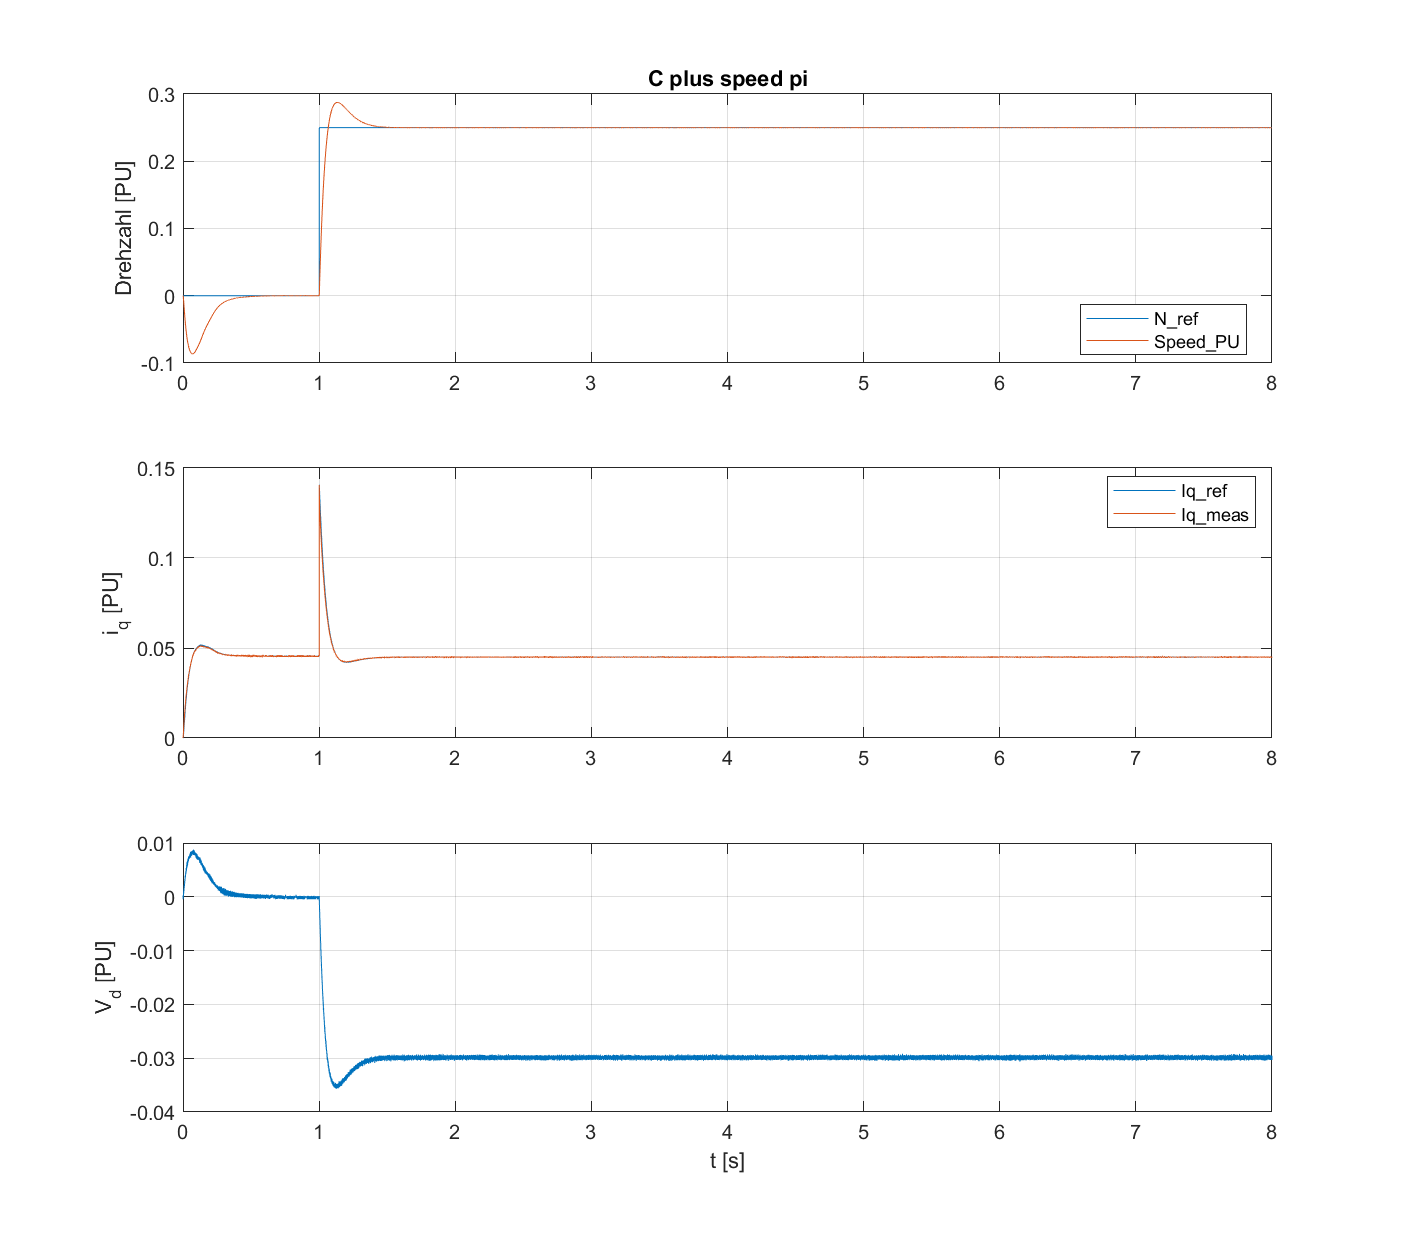
\includegraphics[width=0.9\linewidth]{P1b_C_plus_speed_pi}
  \caption{Stand P1b.1, Lauf C (Strom- und Drehzahlregler korrigiert): Drehzahl, $i_q$ und
    $u_d$ in \ac{PU} bei einem Sollwertsprung auf \SI{0,25}{PU} bei $t = \SI{1}{\second}$
    und \SI{10}{\percent} Lastmoment}
  \label{fig:p1b1}
\end{figure}

Die Ergebnisse sind auch physikalisch plausibel:

\begin{itemize}
  \item \textbf{Lauf A:} Der unkorrigierte Stromregler kann keine negative $d$-Spannung
    stellen, und sein Integralanteil ist praktisch wirkungslos. Der Iststrom bleibt unter dem
    Sollwert, die Drehzahl erreicht nur etwa \SI{0,04}{PU} statt \SI{0,25}{PU}.
  \item \textbf{Lauf B:} Der Iststrom folgt dem Sollwert deckungsgleich. Die bleibende
    Drehzahlabweichung entspricht genau dem P-Verhalten des noch unkorrigierten
    Drehzahlreglers: $i_{q,\mathrm{Last}}/K_p = 0{,}045/0{,}380 = 0{,}118$.
  \item \textbf{Lauf C:} Die Drehzahl folgt dem Sprung mit etwa \SI{15}{\percent}
    Überschwingen und ist nach etwa \SI{0,5}{\second} eingeschwungen, wie für
    $f_c = \SI{5}{\hertz}$ und $T_n = 4/\omega_c$ erwartet. Die anfängliche Abweichung auf
    \SI{-0,09}{PU} entsteht, weil das Lastmoment bereits während der Offsetkalibrierung wirkt,
    in der die Regelung noch nicht arbeitet.
  \item \textbf{$d$-Spannung:} $u_d$ wird mit steigender Drehzahl negativ ($-0{,}015$ bei
    \SI{0,13}{PU}, $-0{,}030$ bei \SI{0,25}{PU}), wie es die Verkopplung
    $u_d \approx -\omega L i_q$ verlangt.
\end{itemize}

Damit erfüllt der Stand P1b.1 die Erwartungen sowohl in den Kennzahlen als auch in den
Zeitverläufen. Er wurde mit dem Tag \texttt{P1b.1} versehen und bildet die Grundlage für die
folgenden Kapitel.

Für die Inbetriebnahme auf der Hardware bleiben zwei Punkte zu beachten. Erstens ist das
Vorzeichen der Strommessung aus dem Schaltplan abgeleitet und sollte vor dem ersten geregelten
Lauf gemessen werden: Ein kleiner Gleichstrom in Phase A muss einen negativen Wert von
$i_{a,\mathrm{PU}}$ ergeben. Zweitens erlaubt die Untergrenze des Drehzahlreglers von $-0{,}5$
ein Bremsen, dessen Energie ein Labornetzteil nicht aufnehmen kann. Beide Punkte werden in
\cref{ch:codegen} und \cref{ch:schutz} behandelt.

\offen{Ergebnis der Vorzeichenmessung auf der Hardware ergänzen bzw.\ auf Hardwareteil verweisen}

\chapter{Verifikation durch Model-in-the-Loop-Tests}
\label{ch:verifikation}

\section{Anforderungen und Tests der Masterarbeit}
% SW_ANF_01/03/04/05; Harnesses Freemode_Check, MaxVel, SpeedController, SafeState
\offen{Text}

\section{Übertragung der Harnesses auf focLib}
% foc_build_harnesses, foc_build_mil_tests, Testdatei focLib_MIL.mldatx
\offen{Text}

\section{Neue Baselines und Toleranzen}
% foc_recapture_baseline, SW_ANF_05 angepasst (A2), Baseline-Abweichung geplottet
\offen{Text}

\section{Ergebnisse}
% 4/4 bestanden für P1a, P1b.1 und nach jeder Folgeänderung
\offen{Tabelle}

\chapter{Codegenerierung und Zielkonfiguration}
\label{ch:codegen}

\section{Codegenerierung für app\_speed}
% slbuild, Fehler der Make-Stufe (NoDefaultCurrentDirectoryInExePath),
% Warnungen, Speicherbelegung (07_Codegen_2026-11-03.md)
\offen{Text}

\section{Takt- und Bausteinkonfiguration}
% externer 25-MHz-Oszillator statt INTOSC2 (für CAN 1 Mbit/s), 200 MHz;
% DeviceID F28386D statt F28388D. Messungen dazu im Hardwareteil.
\offen{Text}

\section{Abgesicherter Build- und Flash-Ablauf}
% Fehler: reines slbuild hat geflasht (08_S5_Fehler_Flash_2026-11-04.md)
% foc_build_action, foc_codegen, foc_flash(model, 'FREIGABE')
\offen{Text}

\chapter{Kommunikation und Diagnose}
\label{ch:kommunikation}

\section{CAN-Anbindung}
% eCAN-A GPIO4/5, 1 Mbit/s, Testmodell, Mailboxen (PVDD 0x110, GVDD 0x111)
\offen{Text}

\section{Protokoll FOCP}
% Bewusste Ausnahme: handgeschriebener C-Code (firmware/focp_c28x.c) als Custom Code,
% Entscheidung dokumentiert in 08_FOCP_Einbau_Plan_2026-11-04.md
% foc_add_focp; INFO/STATUS, Umschaltung Poti/FOC Studio, Sollwerte,
% RX-FIFO und TX-Mailboxen
\offen{Text, Nachrichtenübersicht}

\section{Telemetrie und änderbare Parameter}
% foc_focp_telemetry: 20 kHz, id/iq Ist/Soll, Udc, Hall-Zustand, Temperatur
% foc_tunable_params: Reglerparameter zur Laufzeit aus FOC Studio
\offen{Text}

\section{Fehlersuche: Firmware hängt in der Strom-ISR}
% JTAG-PC-Proben ohne GEL-Reset; Ursache MW_IPC_Write zum CM ohne CM-Programm;
% foc_remove_ipc_cm (08_Fehler_Firmware_haengt_2026-11-05.md)
\offen{Text}

\section{Nicht umgesetzt: UART und External Mode}
% A8 zurückgestellt; Firmware korrekt, Hardwarestrecke offen (Hardwareteil)
\offen{Text}

\chapter{Schutz- und Robustheitsfunktionen}
\label{ch:schutz}
% Je Abschnitt: Anlass (ggf. Hardwarebefund des Laborpartners), Umsetzung
% (Skript, Parameter), Nachweis (test_config, Äquivalenz, MIL, Codegen, Hardware)

\section{Begrenzung des Bremsstroms (A2)}
% ctrl_limits.Iq_min (legacy -0,5 bitgleich, datasheet 0); Rückspeisung ins Labornetzteil
\offen{Text}

\section{Obergrenze des Drehzahlreglers}
% ctrl_limits.Iq_max
\offen{Text}

\section{Rücksetzen der Integratoren im Freemode}
% Stromstoß -31 A beim Freigeben (Windup), reset_I_cur_freemode, Drehzahlregler-Reset
\offen{Text, Telemetrie vorher/nachher}

\section{Sollwert-Totzone}
% Kriechen bei Poti 0, foc_speed_ref_deadband
\offen{Text}

\section{Eingangsqualifikation der Hall-Signale}
% 6 Samples, 500 ns (09_Hall_Qualifikation_2026-11-10.md)
\offen{Text}

\section{ADC-Abtastfenster}
% 300 ns für Ströme, 1 us für langsame Kanäle; Kalibrierblöcke in focLib
% (09_ADC_Abtastfenster_2026-11-10.md)
\offen{Text}

\section{Überspannungsabschaltung}
% 30 V, Hysterese 1 V, im Input Controller (0,2 s); Fehlerbit im FOCP-STATUS;
% Udc_max aus FOC Studio änderbar. Einschränkung: kein schneller Schutz (HW19)
% (09_Ueberspannung_2026-11-20.md)
\offen{Text}

\chapter{PC-Software FOC Studio}
\label{ch:focstudio}

\section{Anforderungen und Bedienkonzept}
% docs/GUI_Entscheidungen.md
\offen{Text}

\section{Architektur}
% host/core (fochost, Qt-frei): Transporte Sim, CANable/gs_usb, SocketCAN, PCAN; Device
% host/studio (Qt 6 Widgets, Qwt); host/app (ImGui, Entwicklerwerkzeug)
% Entscheidung für Qwt nach Plot-Benchmark
\offen{Text, Architekturbild}

\section{Funktionen}
% Übersicht/Dashboard, Parameter (JSON-Import/-Export), Scope, Inbetriebnahme,
% Expertenmodus, Ereignisprotokoll, Deutsch/Englisch
\offen{Text, Screenshot}
% 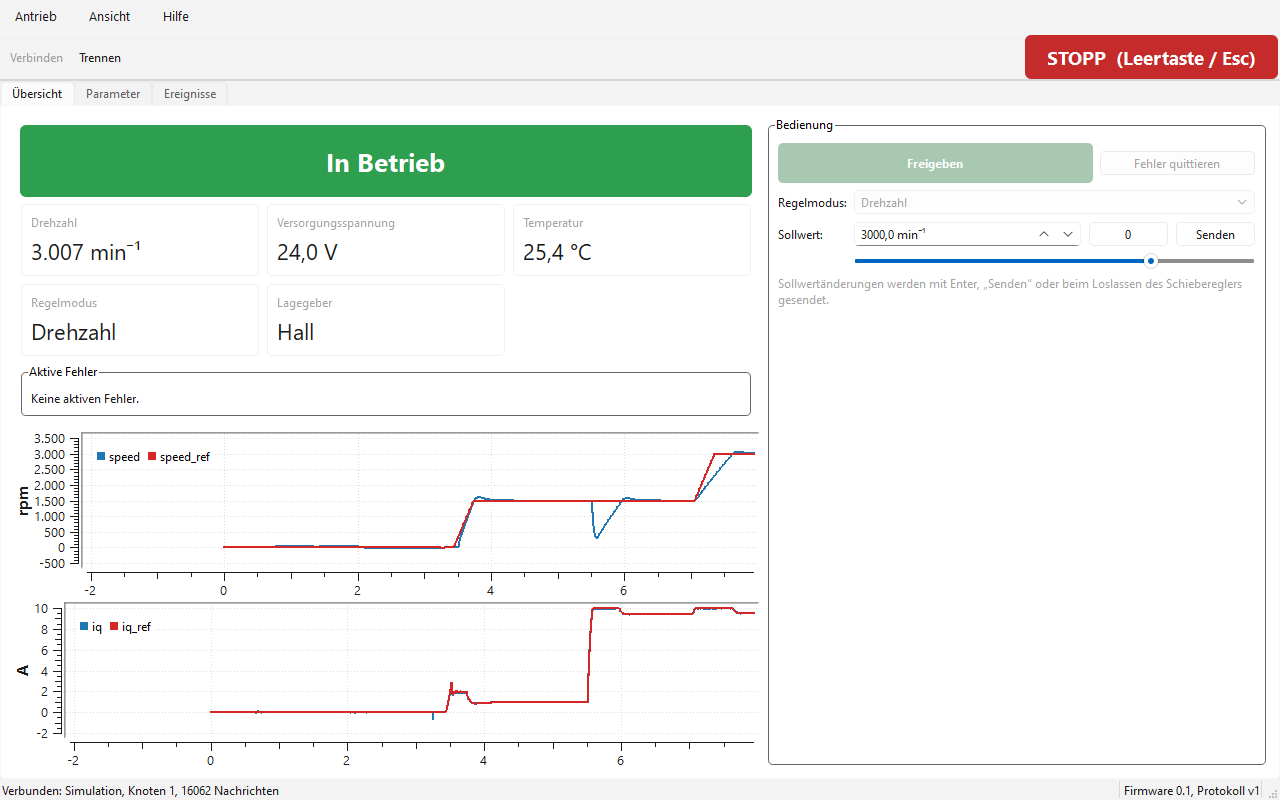
\includegraphics[width=\linewidth]{focstudio_dashboard}

\section{Tests und Auslieferung}
% ctest, virtueller Antrieb (--demo), Installer (NSIS/CPack)
\offen{Text}

\chapter{Zusammenfassung und Ausblick}
\label{ch:fazit}

\section{Zusammenfassung}
\offen{Text}

\section{Offene Punkte}
% A3 dritter Phasenstrom, A4 Überstrom in Hardware (CMPSS/Trip-Zone),
% A5 HAL, A6 Bus-Objekte, A7 Supervisor in Stateflow, A8 UART/External Mode,
% Motoridentifikation (B3)
\offen{Text}


\printbibliography[heading=bibintoc]
\listoffigures
\listoftables

\appendix
\chapter{Modellansichten}
\label{app:modelle}

\begin{sidewaysfigure}
  \centering
  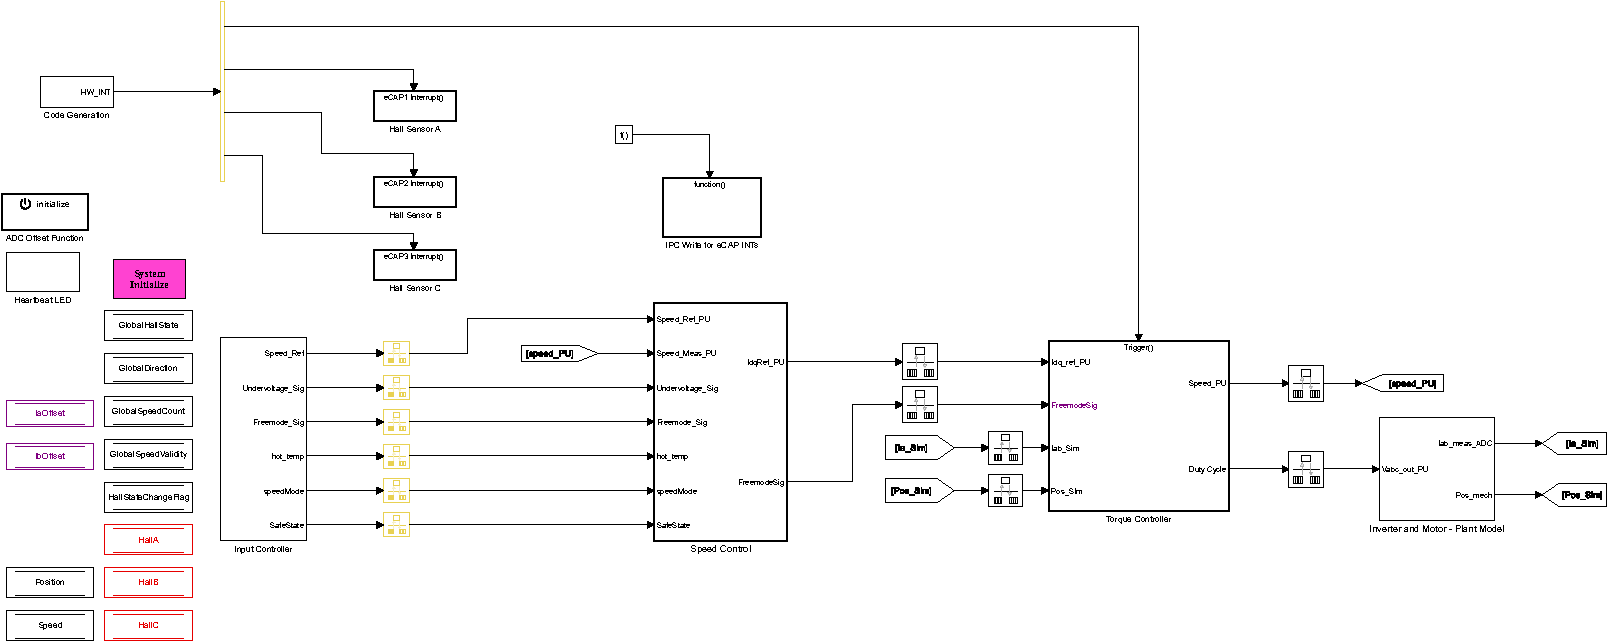
\includegraphics[width=\linewidth]{impmodel_top}
  \caption{Oberste Ebene des Modells \datei{impmodel.slx} aus \cite{akguel2023},
    unveränderte Ansicht aus Simulink}
  \label{fig:impmodel_orig}
\end{sidewaysfigure}

\chapter{Übersicht der Werkzeugskripte}
\label{app:skripte}
% Tabelle matlab/tools/*.m: Skript, Zweck, Schritt/Commit
\offen{Tabelle}

\chapter{Änderungsverlauf}
\label{app:verlauf}
% Tags P1a, P1b, P1b.1 und wichtige Commits mit Kurzbeschreibung
\offen{Tabelle}

\chapter{Konfigurationsparameter}
\label{app:parameter}
% Auszug foc_config: ctrl_limits, PU-Basis, Messkette, Profile im Vergleich
\offen{Tabelle}


\end{document}
